\chapter{Introduction}
Proof assistants, or interactive theorem provers, are tools that help users create and verify formal proofs. Proof assistants like Rocq (formerly Coq) \cite{rocq}, Agda \cite{agda}, and Isabelle \cite{isabelle} have both practical and theoretical applications. Rocq is used to develop and formally verify CompCert \cite{leroy:2009}, a compiler for a large subset of the C programming language and intended for programming reliable embedded systems. In 2005, Georges Gonthier \cite{gonthier:2005} used Rocq to formalise a proof of the four colour theorem, which further clarified doubts about the original computer-assisted proof by Appel and Hakel in 1976 \cite{appel:1976}. Isabelle is used to formally verify the correctness of Transport Layer Security (TLS) \cite{paulson:1999}, a network security protocol.

More recently, proof assistants like Pandora \cite{pandora:2007, pandora}, Carnap \cite{carnap, carnap:2018}, Holbert \cite{oconnor:2022}, and Logitext \cite{yang:2022} have been designed to help students learn logic. They prioritise ease of use over advanced features and help students learn by providing instant feedback on their proofs. Students at Imperial who used Pandora, a proof assistant for Fitch-style \cite{fitch:1952} Natural Deduction, were found to approach exam problems more methodically, were less likely to make arbitrary assumptions, and were more precise in their proofs \cite{pandora:2007}.

However, these educational proof assistants share two key issues:
\begin{itemize}
    \item Each proof assistant supports its own syntax. For example, the universal quantifier ($\forall$) is represented by ``\lstinline{A}'' in Carnap, ``\lstinline{all}'' in Holbert, and ``\lstinline{forall}'' in Logitext. Before students can use the proof assistants, they need to learn unfamiliar syntax which not only does not apply to other proof assistants, but also does not match how they build derivations with pen and paper. This takes away time that could have been spent on learning the proof systems instead.
    \item None of the proof assistants investigated in this report lets users modify proof systems arbitrarily in a user-friendly manner. Among them, Carnap supports the widest range of proof systems, including Natural Deduction for first-order logic \cite{carnap:systems}, the Sequent Calculus \cite{carnap:systems}, and possibly the simply typed $\lambda$-calculus\footnote{The $\lambda$-calculus is not a pre-defined proof system in Carnap. However, Carnap-Core (the libraries which allow users to specify proof systems) supports proof systems with abstractions and applications \cite{carnap:2018}, so it should be able to support the simply typed $\lambda$-calculus.}. However, defining a new proof system, or modifying an old one, requires the user to work with the core libraries in Haskell and cannot be done on the fly.
\end{itemize}

This project presents \projectname{}\footnote{Embla is the first human woman in Norse mythology, mirroring the fact that Pandora is the first human woman in Greek mythology.}, a web-based educational proof assistant that addresses both issues:
\begin{itemize}
    \item Users can build derivations entirely using \LaTeX{} syntax. This means \projectname{} also uses its own syntax, since none of the educational proof assistants above support \LaTeX{}. However, students who already know \LaTeX{} will not need to spend extra time learning unfamiliar syntax, while students who do not know \LaTeX{} will be learning syntax that is useful outside \projectname{}, such as writing assignments and reports.
    \item Users can modify proof systems on the fly without any understanding of the implementation details of syntax and inference rules. Users only need to modify plain text input in the web interface of \projectname{}.
\end{itemize}

\section{Contributions}
The contribution of this project is \projectname{}, a web application with the following features:
\begin{itemize}
    \item Users can define syntax rules (\Cref{section:syntax}) and inference rules (\Cref{section:inference}). \projectname{} supports \LaTeX{} syntax and several shorthand notations. \Cref{fig:introduction:editor} shows what the user sees when editing the syntax and inference rules in \projectname{}.
    \item Users can build derivations in \projectname{}. It verifies whether the derivation is correct according to the syntax and inference rules defined by the user (\Cref{chapter:checking}). Prior to verification, both the inference rules (\Cref{section:inference}) and the derivation given by the user (\Cref{section:term}) are transformed into intermediate internal representations. \Cref{fig:introduction:builder} shows what the user sees when building a derivation in \projectname{}.
\end{itemize}

\begin{figure}[!htbp]
    \centering
    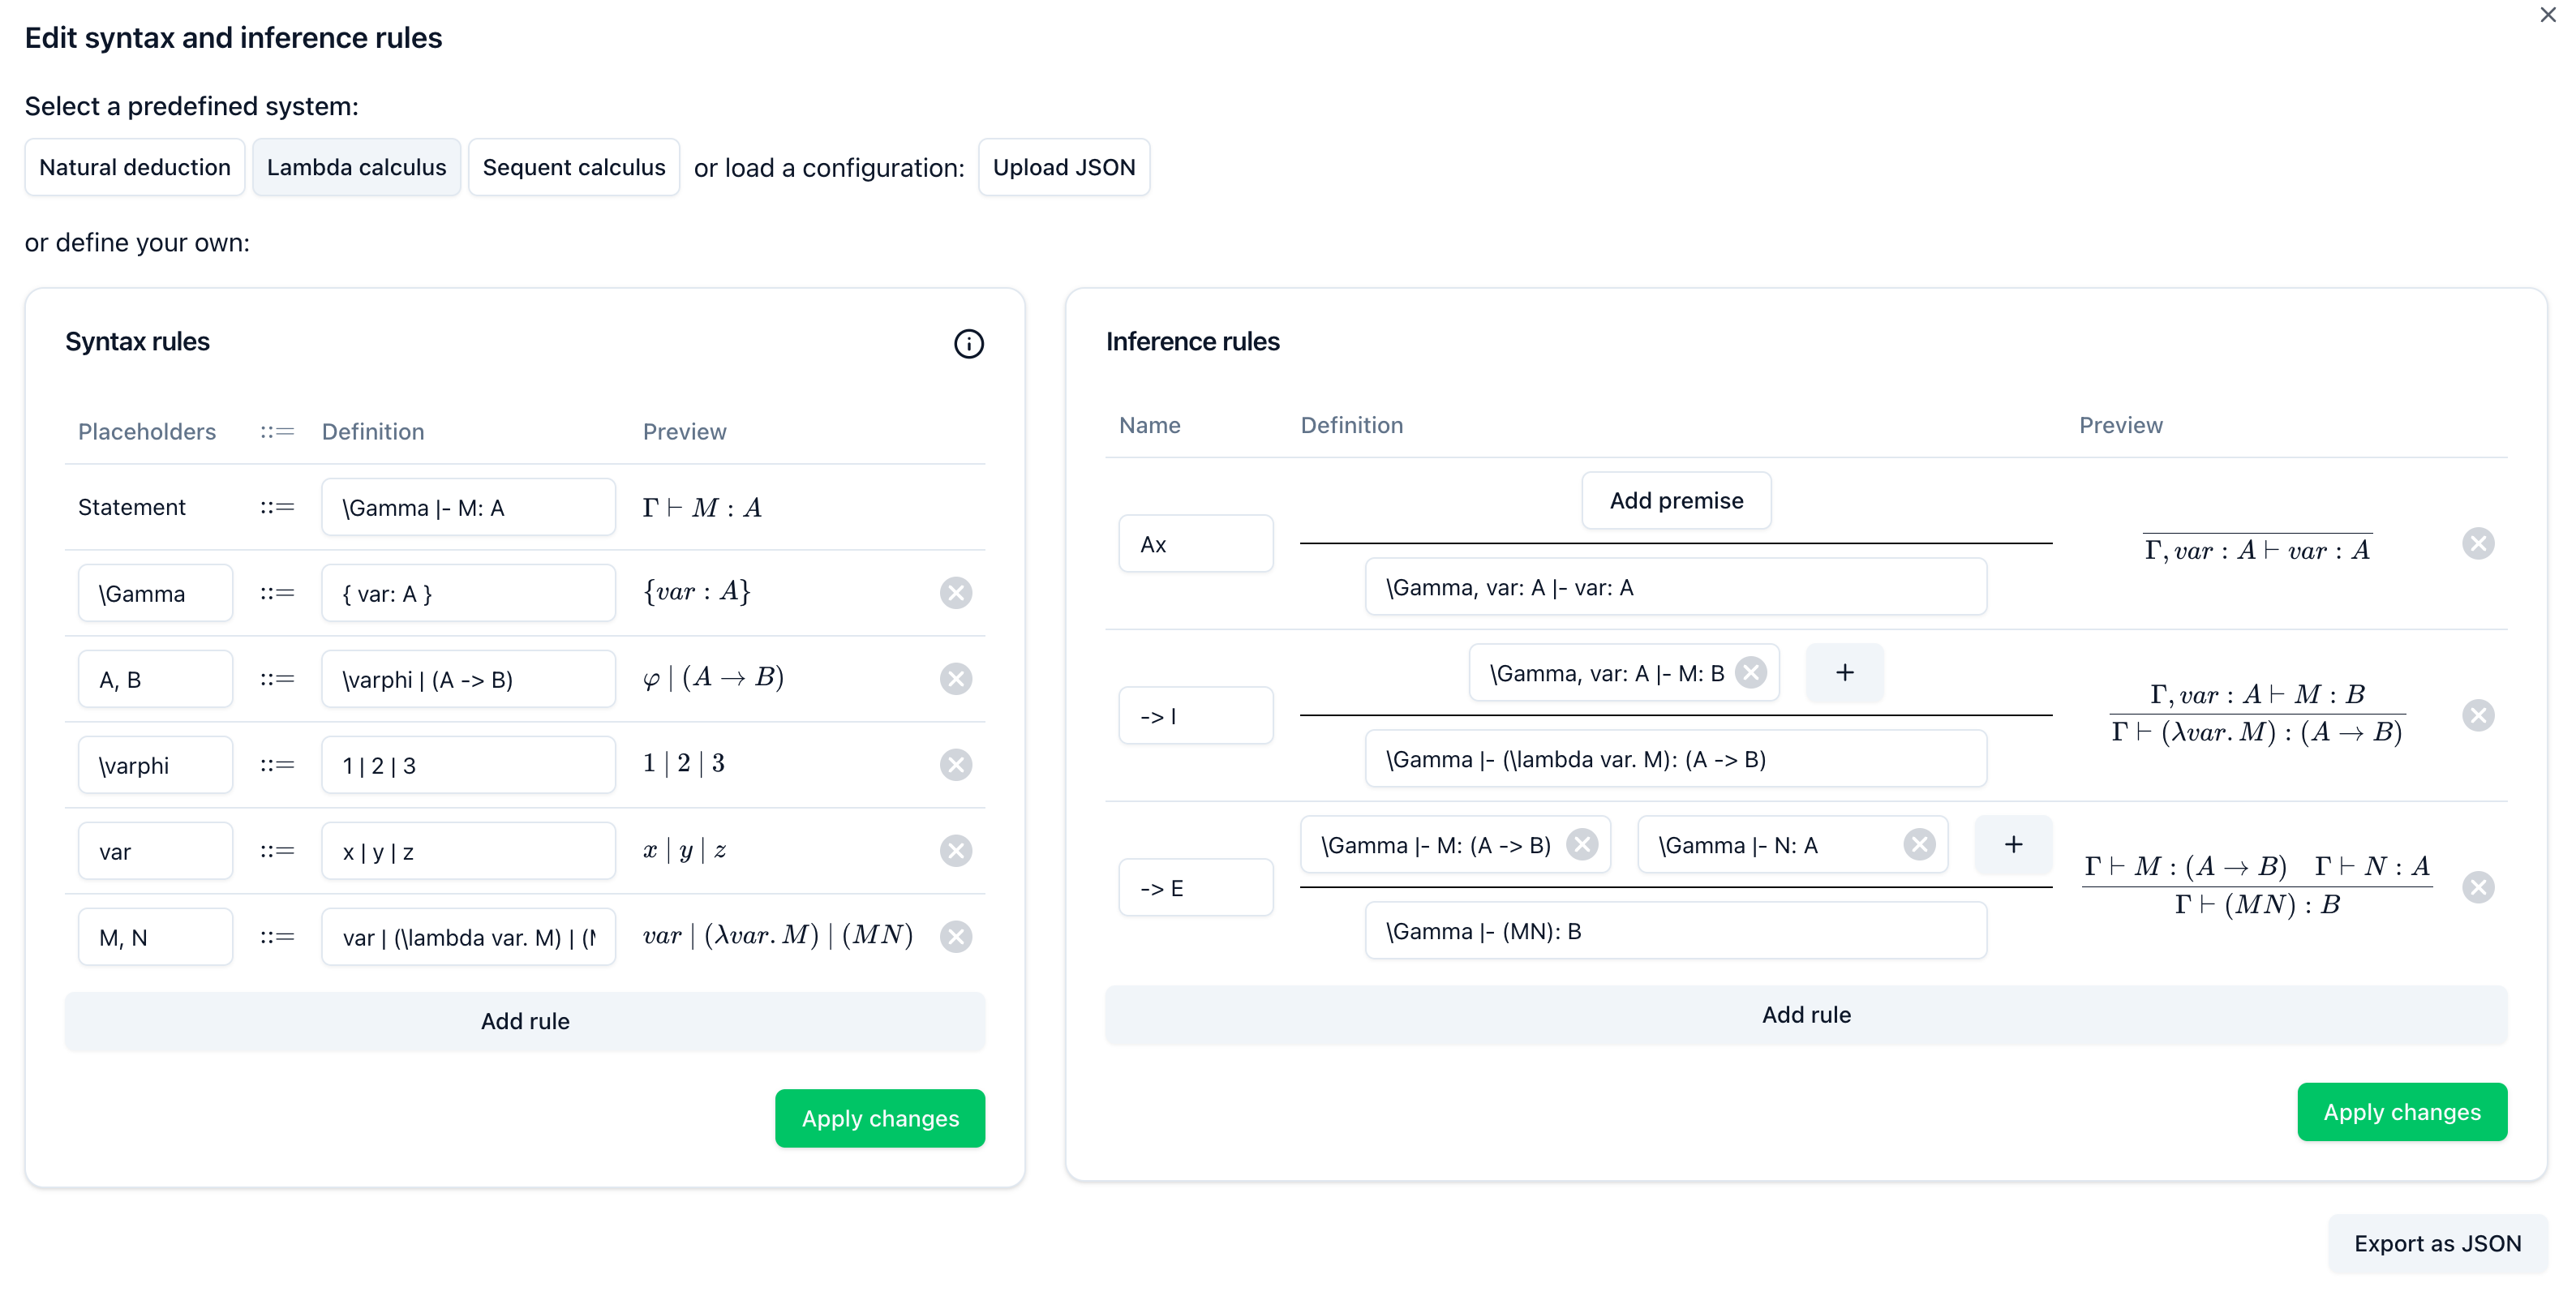
\includegraphics[width=\textwidth]{introduction/editor.png}
    \caption{Editing the proof system in \projectname{}}
    \label{fig:introduction:editor}
\end{figure}

\begin{figure}[!htbp]
    \centering
    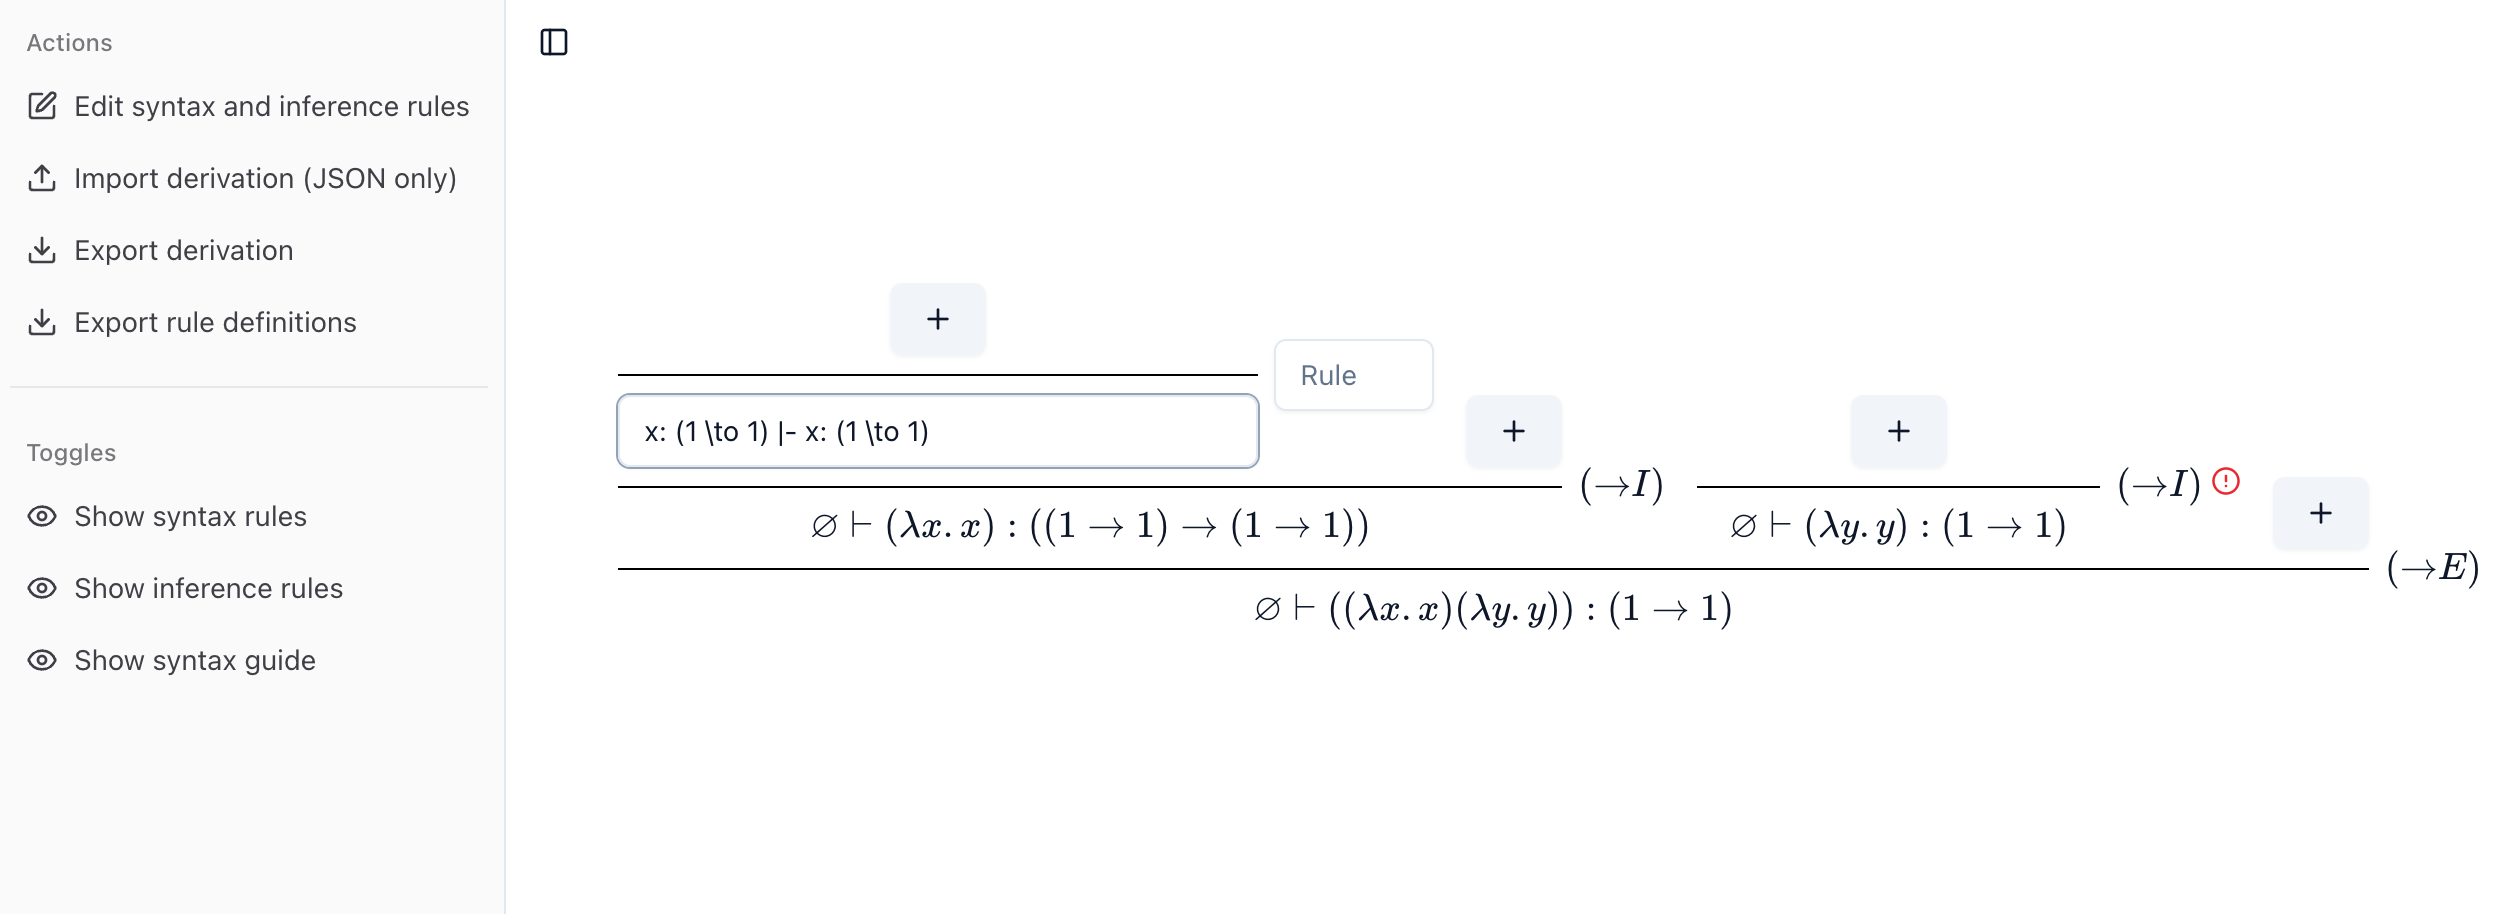
\includegraphics[width=\textwidth]{introduction/builder.png}
    \caption{Building a derivation in \projectname{}}
    \label{fig:introduction:builder}
\end{figure}